
\documentclass{article}
\pdfpagewidth=8.5in
\pdfpageheight=11in
\usepackage{ijcai20}

% Use the postscript times font!
\usepackage{times}
\renewcommand*\ttdefault{txtt}
\usepackage{soul}
\usepackage{url}
\usepackage[hidelinks]{hyperref}
\usepackage[utf8]{inputenc}
\usepackage[small]{caption}
\usepackage{graphicx}
\usepackage{amsmath}
\usepackage{booktabs}
\urlstyle{same}

\title{Hand Gesture Recognition on Arduino Using Photodiodes and Neural Networks}

\author{
Matthew Lipski\\
Supervisors: Mingkun Yang\and
Ran Zhu
\affiliations
EEMCS, Delft University of Technology, The Netherlands\\
\emails
m.s.lipski@student.tudelft.nl,
m.yang-3@tudelft.nl,
r.zhu-1@tudelft.nl
}

\begin{document}

\maketitle

\begin{abstract}
The aim of this template is to make it more clear what is expected from you. 
\textbf{It is by no means required to follow this exact same structure.}
The abstract should be short and give the overall idea:
what is the background, the research questions, what are your contributions, and what are the main conclusions.
It should be readable as a stand-alone text (preferably no references to the paper or to outside literature).
\end{abstract}

%\section{Acknowledgements}\label{sec:acknowledgements}


\setlength{\parskip}{\baselineskip}%
\setlength{\parindent}{0pt}%

\section{Introduction}\label{sec:introduction}
\subsection{Research Overview}\label{subsec:research-overview}
Traditionally, physical buttons have been by far the most common way for users to interact with electronic devices in public settings, whether these are coffee machines, elevator panels, or train ticket machines.
However, the concern of disease transmission has become increasingly prevalent in recent years due to the COVID-19 pandemic, making it enticing to develop an alternative solution which does not require touch.
One such solution is the use of hand gestures to interact with public devices instead.
By performing hand motions such as swiping and tapping, users can effectively and intuitively interact with electronic devices with minimum risk of disease transmission.

However, there are a few key challenges to this approach which stand in the way of it replacing physical buttons in real-world applications.
\begin{enumerate}
    \item Additional hardware is needed to detect the positions of a user's hand while performing a gesture.
    The data output by this hardware is likely to be low in resolution since system costs should be minimized.
    \item Additional software must be implemented to recognize gestures based on hand position over time.
    While buttons are just simple digital inputs, one gesture can also be performed differently between different users, yet the system must be able to accurately classify it regardless.
    \item Gesture recognition must be done in real-time.
    Since the process of classifying gestures can be quite complex, the latency introduced by this may be significant.
    However, the user should not perceive any lag while using the system for a positive experience.
\end{enumerate}

\subsection{Research Question}\label{subsec:research-question}
Given the challenges in developing a neural network for gesture recognition, the goal of this paper can be summarized with the following research question:

\textbf{'Which neural network architecture is most appropriate for recognizing hand gestures on an Arduino Nano 33 BLE, using 3D-formatted data from OPT101 photodiodes?'}

This can then be segmented into the following sub-questions:
\begin{enumerate}
    \item Which neural network architectures produce the highest accuracy for hand gesture recognition?
    \item Which neural network architectures produce the lowest inference latency for hand gesture recognition?
    \item What is the minimum acceptable accuracy for recognizing hand gestures on an Arduino Nano 33 BLE?
    \item What is the maximum acceptable inference latency for recognizing hand gestures on an Arduino Nano 33 BLE?
    \item How can 3D-formatting data be exploited for better gesture recognition performance?
\end{enumerate}

\subsection{Contributions}\label{subsec:contributions}
This research overcomes these challenges by using data from OPT101 photodiodes, which is fed into a neural network to recognize gestures with high accuracy and low latency on an Arduino Nano 33 BLE microcontroller.
It is also part of a larger project which integrates this neural network into a full gesture recognition system, which is elaborated on in section 3.2.

Similar research which involves using photodiodes and machine learning to recognize hand gestures has already been conducted, but this paper improves on existing solutions in a number of ways:
\begin{enumerate}
    \item A high level of accuracy is maintained with fewer photodiodes, and therefore fewer model input features, than existing solutions.
    \item The data from photodiodes is 3D-formatted, which better preserves temporal information and improves recognition accuracy.
    An explanation for what 3D-formatting involves can be found in section~\ref{subsec:3d-formatted-data}.
    \item The neural network used to classify hand gestures is smaller in size than competing solutions, leading to reduced system latency.
\end{enumerate}

A discussion regarding existing research in this field is found in section~\ref{sec:related-work}, which provides more context to these improvements.

%The planned use case for this technology is hands-free navigation of menus which has especially gained relevance due to the restrictions imposed during the COVID-19 pandemic, which has showed that gestures can be an appealing alternative to physical buttons in social settings.
%The most important existing literature for this research comes from Pete Warden and Daniel Situnayake, who are pioneers in the field of embedded AI and authors of the book "TinyML: Machine Learning with TensorFlow Lite on Arduino and Ultra-Low-Power Microcontrollers"\cite{warden2020tinyml}, as well as Qing Wang and Marco Zuniga, who have laid the groundwork for embedded AI specifically in the context of hand gesture recognition\cite{10.1145/3412449.3412551}.
%The research conducted for this paper expands on existing work in this exact way, by using a lower power microcontroller and significantly fewer photo diodes than in the solution created by Wang and Zuniga, while maintaining or improving the classification accuracy of hand gestures.


\section{Background}\label{sec:background}
\subsection{Machine Learning \& Neural Networks}\label{subsec:machine-learning-&-neural-networks}
Machine learning is a sub-field of artificial intelligence which gives a machine the capacity to "imitate the way that humans learn, gradually improving its accuracy" (https://www.ibm.com/cloud/learn/machine-learning).
More specifically, machine learning models "learn" patterns and trends from existing data in order to make accurate predictions on new, unseen data.

Neural networks, meanwhile, are a type of machine learning model which draws inspiration from the human brain.
These types of models feature "neurons" organized into layers, with each layer typically being densely connected to the next.
However, the structure of different neural networks can vary massively, but their main advantage over simpler models is their flexibility and improved ability to deal with highly non-linear data.

\subsection{Machine Learning on Embedded Hardware}\label{subsec:machine-learning-on-microcontrollers}
Machine learning and artificial intelligence have traditionally been restricted to the realms of high-performance and in turn, high power devices.
Unfortunately, this means that it has been previously unfeasible to use these technologies with embedded hardware as it lacks the performance to run machine learning models locally, and lacks the dedicated power to be able to transmit sensor data to a remote processor.
However, recent advances into machine learning model compression and optimization have changed this, allowing deep neural networks to be run on devices even powered by coin batteries, meaning that low-power microcontrollers can make sense of sensor data in much more sophisticated ways than previously possible.

The most prominent development in this field has been TensorFlow Lite for Microcontrollers, which is a Python framework specifically made for running machine learning models on microcontrollers.
The original Tensorflow has been an extremely popular machine learning framework for over a decade, but the extension to make it work effectively on microcontrollers has only been developed in recent years.
Tensorflow, as well as Tensorflow Lite for Microcontrollers, are also specifically designed for developers to work with neural networks rather than other types of machine learning models.

\subsection{Hand Gesture Data}\label{subsec:hand-gesture-data}
In this research, neural networks are used to detect gestures, but to do this, data from some sensor(s) must be fed into the network.
Based on this data alone, it must be possible to distinguish which gesture was performed for the neural network to achieve an acceptable classification accuracy.

There are a variety of sensors which could be used to record hand gestures and provide this data.
One of these is an accelerometer, which lies on the user's wrist (typically from a smartwatch) to track the direction and acceleration of the their hand movements.
Another option is using a camera to record the user's hand, which provides a huge amount of information but is susceptible to noise and requires significantly more intensive processing.
Photodiodes are sensors which output a signal which increases with the amount of light that hits them.
This means they can exploit ambient light by tracking shadows cast by the user's hand, therefore making it possible to recognize which gesture is being performed.
This project uses photodiodes for their much lower cost compared to cameras as well as the fact that they don't require the user to wear a device on their wrists, unlike accelerometers.


\section{System Overview}\label{sec:system-overview}
\subsection{Full Gesture Recognition System}\label{subsec:full-gesture-recognition-pipeline}
This research focuses on finding an appropriate neural network architecture to perform gesture recognition on a microcontroller, but it is only part of a larger project to create an entire gesture recognition system/pipeline.
The creation of this pipeline is composed of the following tasks:
\begin{enumerate}
    \item Optimizing the number and placement of OPT101 photo diodes.
    \item Pre-processing data from photo diodes.
    \item Creating an appropriate dataset for training a neural network to recognize gestures.
    \item Finding an appropriate neural network architecture on the created dataset and ensuring gestures can be recognized in real-time on an Arduino Nano 33 BLE\@.
\end{enumerate}

The research presented in this paper aims to complete task 4.
Although tasks 1--3 were completed by other project group members and are beyond the scope of this research, they are worth mentioning to provide some context regarding the rest of the gesture recognition system.
Due to the findings from these tasks, the final system uses 3 photodiodes and can recognize 10 different gestures, while each gesture is composed of 100 samples from each photodiode.
This is relevant for task 4, as it means that whatever neural network is implemented must use a 2D array of size 3 by 100 (split into \textit{n} frames after 3D-formatting) as an input feature and be able to distinguish between 10 output classes, as illustrated in figure~\ref{fig:system}.

\begin{figure}[h]
    \centering
    \captionsetup{justification=centering}
    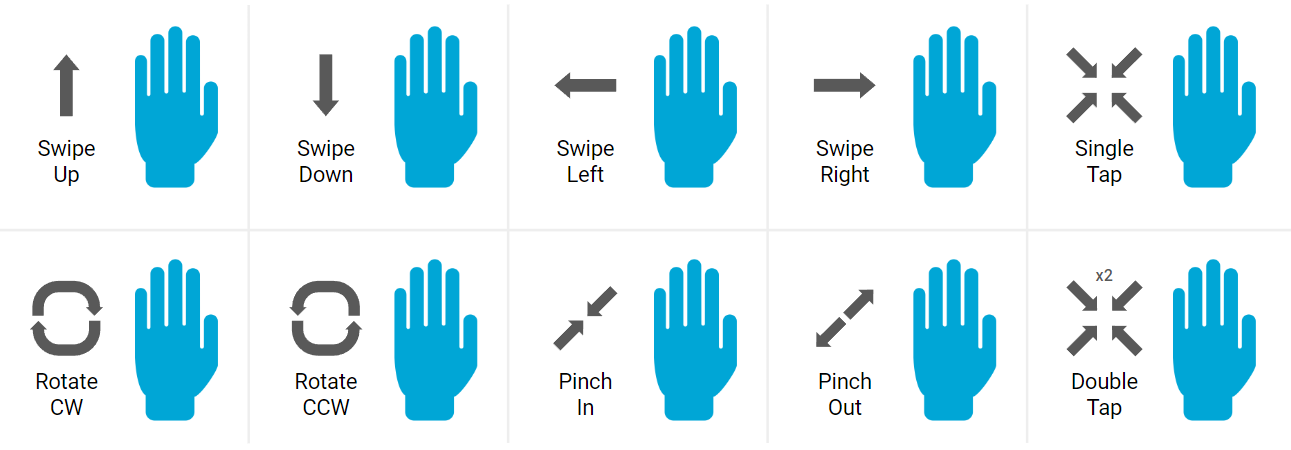
\includegraphics[width=\linewidth]{figures/gestures}
    \caption{Illustrations of the 10 different gestures that the system can recognize.}
    \label{fig:gestures}
\end{figure}

\begin{figure}[h]
    \centering
    \captionsetup{justification=centering}
    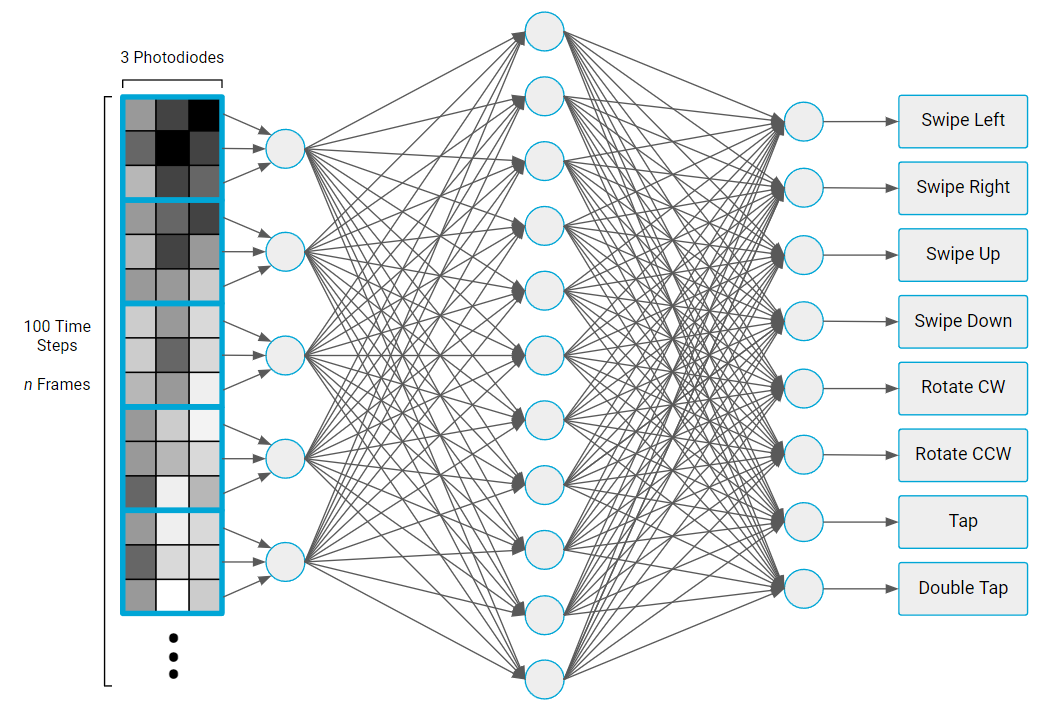
\includegraphics[width=\linewidth]{figures/system_advanced}
    \caption{Visualization of the input features \& output classes using a generic artificial neural network as an example.}
    \label{fig:system}
\end{figure}

\subsection{System Caveats}\label{subsec:system-caveats}
The overarching goal of the project that this research contributes to, is the creation of a full gesture recognition pipeline, which presents some issues when considering the fact that each part of this pipeline was developed in parallel.
In reality, it would make much more sense to complete each step of the pipeline sequentially, as the performance of later parts of the pipeline relies on the performance of previous parts.
To put this in the context of the gesture recognition system, it is impossible to train a neural network to recognize gestures without first having a dataset to train it on.
However, the creation of that dataset relies on photodiode count and placement, as well as sampling rate and pre-processing, being finalized.
If they change after the dataset is completed, it will not be representative of real-world data, leading to poor gesture classification performance from the neural network trained on it.

\subsection{Dataset}\label{subsec:dataset}
Having a varied, expansive, and representative dataset is crucial for training a machine learning with high real-world accuracy.
Fortunately, a dataset for recognizing gestures using photodiode data was done by another member of the project group, as mentioned in section~\ref{subsec:full-gesture-recognition-pipeline}.

Unfortunately, because the allotted time for the project meant that all group members had to work in parallel, as stated in section~\ref{subsec:system-caveats}, the neural networks evaluated in this paper had to be trained on a dataset that is not final.
Specifically, the dataset used in this research is not passed through the data pre-processing stage of the system.
This means that the neural networks presented in this paper were trained on raw data from the photodiodes, whereas real-world data on the final system would include this pre-processing step.
This leads to accuracy measurements being lower than they could be, as there is noise and other artifacts in the raw photodiode data.

The dataset used contains 5 repetitions of each of the 10 gestures per hand across 48 participants, leading to 4800 total data instances.
Each instance is made up of a 5 second window during which a gesture is performed over the photodiodes, with a sampling rate of 20Hz for a total of 100 samples per photodiode.
Although the dataset contains instances from a variety of environments and lighting setups, these are mostly indoor locations as this is the planned use case for the system.
The dataset was also mostly recorded on the TU Delft campus, meaning the demographic of participants is somewhat skewed.
Most notably, the dataset contains substantially more instances of males compared to females, and more right-handed participants than left-handed.
However, this is not expected to have a large impact on the performance on any neural networks trained on this dataset.

\section{Model Design}\label{sec:model-design}
\subsection{Neural Network Architectures Tested}\label{subsec:architectures-tested}
Recognizing hand gestures based on photodiode data can be thought of as a time-series classification task, which is a type of problem that recurrent neural networks (RNNs) are especially well suited for~\cite{HUSKEN2003223}.
RNNs differ from conventional neural networks as they do not process the input in its entirety, but instead process each time step or sample from the input sequentially.
Each time step is used to update a "hidden state", which is fed back into the RNN along with the next time step.
This gives RNNs the ability to exploit the time-sensitive nature of time-series data, as each time step also has temporal information associated with it.
Thanks to this desirable property, RNNs were the first type of neural network tested.

Although RNNs are highly suitable for time-series classification, they suffer from the "vanishing gradient problem", which has since been overcome by long short-term memory cells (LSTMs) and gated recurrent units (GRUs)~\cite{DBLP:journals/corr/abs-1801-06105}.
To briefly explain this problem, the weight of the hidden state of a time step in an RNN tends to exponentially decrease for future time steps.
This means that in practice, RNNs tend to ignore if earlier time steps are out of order, which limits performance for long data sequences.
LSTMs and GRUs solve this issue using so-called "gates", which determine which contents of the previous hidden state should be kept and which contents of the current hidden state should be propagated to the next time step.
This largely mitigates the vanishing gradient problem as only relevant information is kept, therefore greatly reducing the rate at which hidden state weights decay.
Given that LSTMs and GRUs are should yield better classification performance than RNNs due to this advantage, these were also investigated.

One issue of using LSTMs and GRUs, however, is that they only accept a single data sequence with multiple features as input, in which each time step contains a single value from each feature, i.e.\ a 1D array.
This is relevant as with 3D-formatted data, each time step is a 2D frame - not a 1D array.
Therefore, each frame has to be flattened first, which causes a loss of spacial information.
This issue can be solved by using a convolutional neural network (CNN) to remove noise from the input data and extract features, which are then fed into the LSTM~\cite{KIM201972}.
CNNs accept 2D images as input, which means that frames do not have to be flattened.
By using convolutional and pooling layers, the resolution of this image can be reduced to just a single value for each neuron in the final layer of the CNN\@.
Therefore, the final CNN layer effectively outputs a 1D array with a size equal to the number of neurons in it, which can then be used as input to the LSTM with no loss in spacial information.
Due to this, the CNN-LSTM architecture was also investigated in this study.

Finally, transformer encoders were also tested for this project as a novel alternative to RNN based architectures.
Transformers use a concept called self-attention which identifies which elements in a sequence carry most semantic value based on the other elements of the sequence~\cite{https://doi.org/10.48550/arxiv.1706.03762}
This is fundamentally different to the hidden state mechanism used by RNNs and their derivatives.
They are typically used in language translation and are made up of two parts, an encoder and a decoder.
The encoder converts the input into an internal representation, which can then be manipulated and decoded into a more useful format, while the decoder converts this internal representation back into a more useful data type.
In a study by Y{\"u}ksel \textit{et al.}~\cite{yuksel-etal-2019-turkish}, a transformer encoder was used to classify topics from sequences of Turkish text taken from Twitter.
Although this is clearly different to the goal presented in this paper, i.e.\ classifying gestures based on photodiode readings, both are classification tasks using input data in which order is important.
Given the positive results found in this study, it seemed reasonable to test transformer encoders for gesture recognition as well.

\subsection{Parameter Tuning}\label{subsec:frame-size}
When training a machine learning model, the model parameters can have a substantial impact on final performance.
For the neural networks tested in this paper, some of these parameters affect almost all model types, while some are specific to individual architectures.
These are outlined below:

\subsubsection{All Architectures}
\begin{itemize}
    \item Frame size
    \item Number of layers
    \item Number of neurons per layer
\end{itemize}

\subsubsection{CNN+LSTM}
\begin{itemize}
    \item Number of convolutional layers
    \item Number of neurons per convolutional layer
    \item Filter kernel sizes
\end{itemize}

\subsubsection{Transformer Encoder}
\begin{itemize}
    \item Number of attention heads
\end{itemize}

In reality, there are more parameters that could be tuned, but the ones listed above are likely to have the largest impact on final model performance.
This paper does not go into detail regarding the testing of different parameters to determine which combinations yield optimal performance, but the final parameter values are stated in section~\ref{subsec:accuracy-testing-results}.


\section{Model Implementation}\label{sec:model-implementation}
\subsection{Accuracy Testing}\label{subsec:validation-accuracy-testing}
To ensure that the measured validation accuracy for a given architecture was as high as possible, as well as being representative of real world performance, four distinct measures were put in place.
The first of these was the addition of a dropout layer with $p=0.5$, before the output layer, to ensure that overfitting would not be an issue~\cite{JMLR:v15:srivastava14a}.
The second measure was%CFR$ S the use of k-fold cross-validation~\cite{inbook} with $k=10$, as validation accuracy can be skewed based on how the test and validation sets are split.
Thirdly, each model architecture was trained until the value of the loss function did not improve after 200 consecutive epochs.
Once training was complete, the model weights were also reverted to the epoch after which the loss function value was lowest.
This removes the variance caused by randomizing initial model weights as well as differences in model training time, and allows each model to achieve close to its maximum possible performance.
Finally, the dataset was shuffled randomly before each model was validated as ordered data can cause anomalies with training and k-fold cross-validation.

\subsection{Latency Testing}\label{subsec:latency-testing}
TODO

\subsection{Codebase}\label{subsec:testing-framework}
The implementation and testing of each model architecture was done using the TensorFlow Python library and high-level Keras API\@.
The models were converted to TensorFlow Lite and C to be used for inference on an Arduino Nano 33 BLE as detailed in chapter 4.5 of "TinyML Machine Learning with TensorFlow Lite on Arduino and Ultra-Low-Power Microcontrollers"~\cite{warden2020tinyml}.
All code used for this research can be found at https://github.com/matthewlipski/research\_project.

\section{Results}\label{sec:results}
\subsection{Inference Latency Testing}\label{subsec:inference-latency-testing}
\subsubsection{Methodology}
Unfortunately, it is not currently possible to test the inference latency performance of most neural networks architectures tested directly on the Arduino Nano 33 BLE\@.
As mentioned in section~\ref{sec:model-implementation}, the TensorFlow library is used to train the neural networks, while TensorFlow Lite for Microcontrollers is used run inference on them.
However, the Arduino implementation of TensorFlow Lite for Microcontrollers does not currently have support for recurrent neural networks, which are also needed for all other architectures tested excluding transformer encoders.
While it is possible to use RNNs with the most recent version of TensorFlow Lite for Microcontrollers (version 2.9), the library's Arduino implementation is a few versions behind (currently version 2.4), and is outdated enough that it is missing certain tensor operations necessary for running RNNs and their derivatives.

Therefore, a different method was used to estimate the inference latency of RNNs on Arduino.
Since regular artificial neural networks are compatible with TensorFlow Lite for Microcontrollers version 2.4, several configurations of these with varying neuron and densely connected layer counts were trained and deployed on the Arduino Nano 33 BLE\@.
These configurations are listed in table~\ref{tab:ann_configs}, formatted as (number of densely connected layers layers/number of neurons per layer).
Each configuration also includes a final densely connected layer of 10 neurons for output.
Since ANNs require 1D input data, a dummy data instance was taken from the dataset and flattened into a single array of 300 values (3 photodiodes $\times$ 100 samples).
This dummy data instance was then used as input to the networks so that their latencies could be measured.
The inference times of these generic networks on the Arduino Nano 33 BLEs were compared to their TensorFlow Lite file (.tflite extension) sizes, to see if file size could be used to predict inference latency.

\begin{table}[]
    \centering
    \captionsetup{justification=centering}
    \begin{tabular}{lll}
        Configuration & File Size (MB) & Latency (ms) \\
        \hline
        (1/128)       & 42             & 103.9        \\
        (1/256)       & 81             & 179.6        \\
        (1/512)       & 160            & 333.0        \\
        (2/64)        & 27             & 74.7         \\
        (2/128)       & 59             & 134.5        \\
        (2/256)       & 147            & 293.7        \\
        (4/32)        & 17             & 55.4         \\
        (4/64)        & 59             & 92.3         \\
        (4/128)       & 93             & 195.0
    \end{tabular}
    \caption{Table comparing the file sizes and inference latencies of various TensorFlow Lite artificial neural networks.}
    \label{tab:ann_configs}
\end{table}

\subsubsection{Results}
Figure~\ref{fig:latency_results}\@ illustrates that a neural network's inference latency can indeed be estimated using the function $y = 1.89x + 23.6$, where $x$ is the model file size in kilobytes and $y$ is the model's expected inference latency in milliseconds.

\begin{figure}[h]
    \centering
    \captionsetup{justification=centering}
    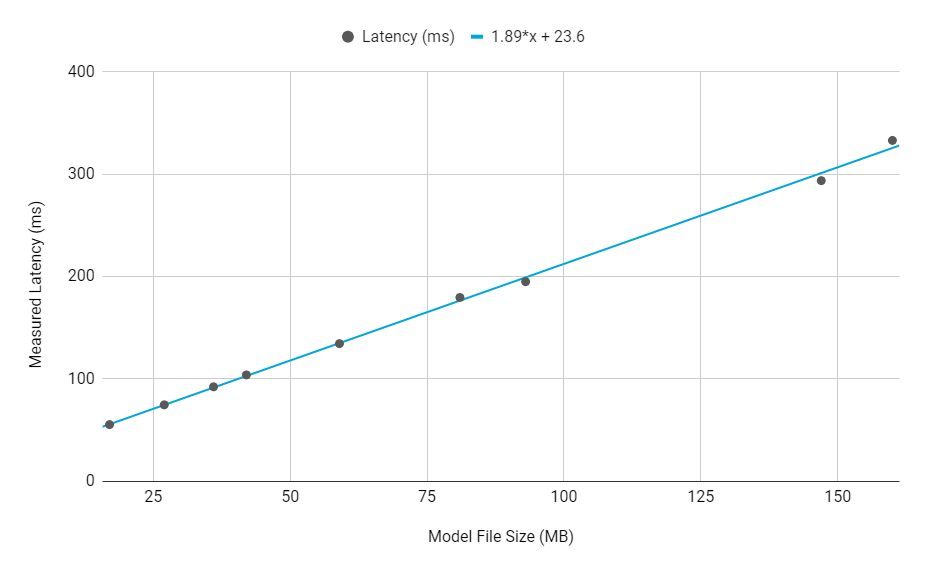
\includegraphics[width=\linewidth]{figures/latency_results}
    \caption{Graph showing the relationship between file size and inference latency for various TensorFlow Lite artificial neural networks.}
    \label{fig:latency_results}
\end{figure}

However, it is worth noting that the largest model for which latency was tested, with a 160KB file size, only produced a latency of 333 milliseconds despite using 97\% of the available RAM on the Arduino Nano 33 BLE (this memory usage includes the boilerplate code needed for loading and running the model).
A latency of 333ms is similar to human reaction time (CITATION NEEDED) and can therefore be considered real-time for the purpose of gesture recognition.
Therefore, inference latency is not much of a concern, though it is important that all models tested in this study do not exceed a file size of \~160KB, so that they could be run on the Arduino in the future.

\subsection{Accuracy Testing}\label{subsec:accuracy-testing}
\subsubsection{Methodology}
To ensure that the measured validation accuracy was representative across all neural network architectures tested, four distinct measures were put in place:
\begin{enumerate}
    \item A dropout layer with $p=0.5$ was added before the output layer for each architecture to reduce overfitting~\cite{JMLR:v15:srivastava14a}.
    \item K-fold cross-validation~\cite{inbook} was used with $k=5$, as validation accuracy can be skewed based on how the test and validation sets are split.
    \item Each neural network was trained until the value of the validation function no longer improved for 100 consecutive epochs, mitigating the variation in training time caused by randomizing initial neuron weights as well as differences in architecture.
    \item Data instances for each participant in the dataset were shuffled randomly, as ordered data can cause slow training times and poor performance.
    However, the order of participants was not shuffled to ensure that gestures in the training data were recorded by different participants to gestures in the validation data, making validation more representative of a real-world scenario.
\end{enumerate}

\subsubsection{Results}

\subsubsection{RNN}

\subsubsection{LSTM}

\subsubsection{GRU}

\subsubsection{CNN+LSTM}

\subsubsection{Transformer Encoder}


\section{Related Work}\label{sec:related-work}


\section{Responsible Research}\label{sec:responsible-research}
All code used for this research is open source can be found at https://github.com/matthewlipski/research\_project.
Due to the inherent randomness present when training neural networks, the results presented in this paper may not be completely reproducible.
However, using the same code and hardware, it should be possible for anyone to reach the same conclusions based on their own findings.
The code being open source also allows others to find potential flaws in it, allowing it to be worked on and used for future research.

The work conducted for this study was also heavily focused on experimentation rather than reviewing literature.
Naturally, research into existing work was still required to provide a starting point for testing and find which neural network architectures would be most suitable for recognizing gestures, as well as find potential improvements to existing work.
However, this emphasis on testing and experimentation rather than reading literature means that the testing methodology falls under the under most scrutiny, and that ensuring the results of this research are reproducible is paramount.
This is why much of the paper is devoted to explaining the system and testing setup.
Although it may seem overly detailed at times, it is crucial to go over the methodology in depth in order for the results presented in this study to be reproducible.


\section{Conclusion}\label{sec:conclusion}


\bibliographystyle{plain}
\bibliography{references}

%A rule of thumb for dealing with the literature is the following: scan about 10--20 contributions: read title, abstract, part of introduction and conclusions; categorize contribution; some of these are studied in more depth: completely read about 5 conference papers or equivalent (summarize contribution in own words); of which studied in-depth about 2 conference papers (the student is able to explain in detail and criticize contributions). This may result in 5--20 references, possibly even more if the project is a literature study.


\end{document}

